\documentclass[10pt, xcolor=x11names]{beamer}
%\usecolortheme{seagull}
\useoutertheme{infolines}
\usefonttheme[onlymath]{serif}
\setbeamertemplate{headline}[default]
\setbeamertemplate{navigation symbols}{}
\mode<beamer>{\setbeamertemplate{blocks}[rounded][shadow=true]}
\setbeamercovered{transparent}
%\setbeamercolor{block body example}{fg=blue, bg=black!20}

\usepackage[utf8]{inputenc}
\usepackage[]{csquotes}
\usepackage{amsmath}
%\usepackage{tikz, wasysym}
%\usepackage{graphicx}
%\usetikzlibrary{automata,positioning}
%\usepackage{hyperref}
%\usepackage{amsfonts}
%\usepackage{csquotes}
%\usepackage{tikz}
%\usetikzlibrary{arrows}
%\usetikzlibrary{arrows.meta}
%\usetikzlibrary{positioning}
%\usepackage{wrapfig}
%\usepackage{pgfplots}
%\usepackage{outlines}
%\usepackage{mathtools}
%\usepackage{xcolor}
%\usepackage{amsfonts}
%\usepackage{amssymb}
%\usepackage{makeidx}
%\usepackage{graphicx}


\usepackage{hyperref}
\author{Sven Fiergolla \& Tobias Dahlem}
\title[]{btrfs \& F2FS vs. ext4}
\subtitle[short version]{}
\date{3. März 2020}
%\institute[Uni Trier]{Universität Trier}
%\logo{\includegraphics[scale=.25]{unilogo.pdf}}

\begin{document}
	
	\frame{\maketitle}
	\frame{\frametitle{}
		\tableofcontents
	}
	
	\section{Introduction - Flash memory}
	\frame{\frametitle{Besonderheiten des Flashspeichers}
		\begin{itemize}
			\item Adressen Mapping
			\begin{itemize}
				\item Zuweisung von logischen zu physischen Adressen
				\item Häufige Verwendung wegen Charakteristika von Flash-Speichern
			\end{itemize}
			
			\item Garbage Collection
			\begin{itemize}
				\item Alte Daten/Seiten werden als ungültig markiert (Allokierter Speicherplatz)
				\item Hoher Aufwand durch kopieren von Blöcken
			\end{itemize}
			
			\item Wear Leveling
			\begin{itemize}
				\item Begrenzte Haltbarkeit von Flash-Zellen (Löschen, Schreiben)
				\item Gleichmäßige Abnutzung der Zellen
			\end{itemize}
			
			\item[ ]
			
			\item Verwendung eines Flash Translation Layer (FTL) im Controller
		\end{itemize}
	}
	
	\section{btrfs}
	\frame{\frametitle{btrfs}
		
	}
	
	\frame{\frametitle{btrfs - Struktur}
		
	}
	
	\frame{\frametitle{btrfs - CoW}
		
	}
	
	\frame{\frametitle{btrfs - RAID}
		
	}
	
	\section{F2FS}
	\frame{\frametitle{F2FS}
		\begin{itemize}
			\item Flash-Dateisystem von Samsung (veröffentlicht 2012)
			\item Entwickelt nur für Flash-Speicher (SD-Karte, SSDs, eMMC-Karten)
			\item Ziel: Optimierung der Performance und Lebenszeit von Flash-Speichern
			\item Entwickelt als Open-Source Projekt
			
			\item[ ] 
			\pause\item Verfolgt den Ansatz eine Log-structured File System (append-only logging)
			\item Arbeitet nicht auf ,,raw'' Flash-Zellen (Benötigt einen FTL)
			\item Viele Möglichkeiten zur Anpassung des Systems
			\item Verwendung von iNodes und Datenblöcken (Ähnlich zu UNIX)
			
			\item[ ] 
			\pause\item Verfügbar ab Linux Kernel 3.8  
			\item Verwendung in Huawei (2016), Galaxy Note 10, Google Nexus
		\end{itemize}
	}
	
	\frame{\frametitle{F2FS - Flash-friendly on-disk Layout}
		\begin{itemize}
			\item Orientierung an FTL-Einheiten um Kosten zu Vermeiden
			\item Einheiten: Blöcke, Segmente, Sektionen, Zonen
			\pause\item Metadaten: 
			\begin{itemize}
				\item Random Writes: Vorhalten in Arbeitsspeicher (Bei Checkpoints schreiben)
			\end{itemize}
			\pause\item Haupt-Speicherbereich:
			\begin{itemize}
				\item Aufgeteilt in Standardmäßig 4KB Blocks (Jeder Block ist Node- oder Data-Block)
				\item Node- und Data-Blocks liegen in verschiedenen Segmenten
			\end{itemize}
		\end{itemize}
		\pause
		\visible<2->{
			\begin{figure}[h]
				\centering
				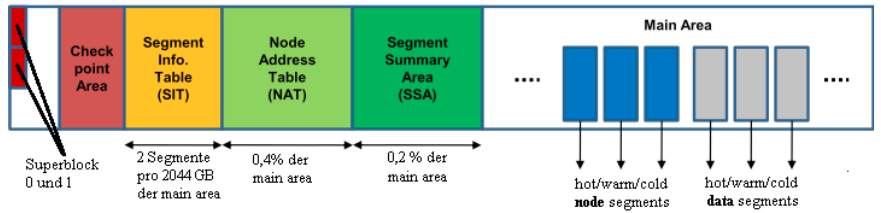
\includegraphics[width=\textwidth]{Figure_F2FS_ODL.png}
				\caption{on-disk Layout F2FS}
			\end{figure}
		}
	}
	
	\frame{\frametitle{F2FS - Besonderheiten I}
		\begin{itemize}
			\item Multi-Head Logging
			\begin{itemize}
				\item Mehrere aktive Logsegmente parallel (Standard 6) 
				\item Parallele Verwendung durch Architektur möglich (multi-Streaming Interface)
				\item Unterscheidung der Daten in hot/warm/cold Schema (Update Frequenz)
			\end{itemize}
			
			\pause\item Kosten-Effiziente Index Struktur
			\begin{itemize}
				\item Verwendung einer neuartigen Indexes: note adress table (NAT)
				\item Zur Vermeidung des ,,wandering tree'' Problems 
				\begin{itemize}
					\item Nur Update des direct Node Block und NAT
					\item Reduktion der Updates um Schreiboperationen zu sparen 
				\end{itemize}
			\end{itemize}
			
			\pause\item Adaptive logging
			\begin{itemize}
				\item Append-only Logging : Standardmäßig (random writes werden sequentiell)
				\item Threaded Logging : Verwendung bei hoher Auslastung (random writes)
			\end{itemize}
		\end{itemize}
	}
	
	\frame{\frametitle{F2FS - Besonderheiten  II}
		\begin{itemize}
			\item Garbage Collection
			\begin{itemize}
				\item On-Demand: Wenn nicht genügend Speicherplatz verfügbar ist
				\begin{itemize}
					\item Greedy: Auswahl des Opfersegments mit wenigsten gültigen Blöcken
				\end{itemize}
				\item Background: Bei geringer Auslastung des Systems von Kernel ausgeführt
				\begin{itemize}
					\item Kosten-Effizient: Auswahl durch Segment-Alter und Anzahl gültiger Blöcke
				\end{itemize}
			\end{itemize}
			
			\pause\item RAID
			\begin{itemize}
				\item In Progress ...
			\end{itemize}
		\end{itemize}
	}
	
	\frame{\frametitle{F2FS - Bewertung}
		
		\begin{itemize}
			\item Vorteile
			\begin{itemize}
				\item Optimierung der Zusammenarbeit von FTL und Dateisystem
				\item Vermeidung des Wandering Tree Problems
				\item Anpassung des Dateisystems an System-Status
				\item Hohe Anzahl an Parametern um Dateisystem anzupassen
			\end{itemize}
			
			\pause\item Nachteile
			\begin{itemize}
				\item Nur für Flash-Speicher (mit einem FTL)
				\item FTL Qualität wichtiges Kriterium 
				\item Initialer hoher belegter Speicherplatz durch Metadaten
				\item Hohe CPU-Belastung beim Schreiben von Dateien
			\end{itemize}
		\end{itemize}
		
	}
	
	\section{benchmarks}
	\frame{\frametitle{benchmarks}
		
	}
	\frame{\frametitle{benchmarks - Results}
		\begin{table}[h]
			\begin{tabular}{r|r|r|r|r|r}
				
			\end{tabular}
			\label{tab:t100benchmark}
			\caption{Benchmark}
		\end{table}
	}
	
	
	
	
	
	
	
\end{document}
